\documentclass[11pt,a4paper]{article}

\usepackage[margin=1in]{geometry}
\usepackage{amsmath,amssymb,amsfonts,mathtools}
\usepackage{bm}
\usepackage{physics}
\usepackage{tikz}
\usetikzlibrary{arrows.meta, positioning, fit, shapes.geometric, calc, decorations.pathmorphing, backgrounds}
\usepackage{caption}
\usepackage{subcaption}
\usepackage{array}
\usepackage{booktabs}
\usepackage{enumitem}
\usepackage{xcolor}
\usepackage{listings}
\usepackage[most]{tcolorbox}
\usepackage{hyperref}
\usepackage{fancyhdr}
\usepackage{graphicx}
\usepackage{float}

% ============================================================================
% COLOR PALETTE -- Isaac Sim orange/black theme
% ============================================================================
\definecolor{isaacorg}{RGB}{220,120,20}
\definecolor{isaacdark}{RGB}{40,40,50}
\definecolor{isaacgreen}{RGB}{40,160,60}
\definecolor{isaacblue}{RGB}{50,120,200}
\definecolor{isaaccyan}{RGB}{0,170,190}
\definecolor{darkred}{RGB}{180,30,30}
\definecolor{resultbg}{RGB}{230,255,230}
\definecolor{resultbar}{RGB}{40,140,60}
\definecolor{warnbg}{RGB}{255,245,220}
\definecolor{warnbar}{RGB}{200,140,0}
\definecolor{lightgray}{RGB}{245,245,245}
\definecolor{physxpurple}{RGB}{130,60,180}

% --- Equation-after-code box ---
\definecolor{eqboxbg}{RGB}{255,248,236}
\definecolor{eqboxbar}{RGB}{200,120,20}
\definecolor{eqboxlabel}{RGB}{180,100,10}

\newtcolorbox{codemath}{%
    enhanced,
    breakable,
    colback=eqboxbg,
    colframe=eqboxbar,
    boxrule=0pt,
    leftrule=3.5pt,
    arc=0pt,
    outer arc=0pt,
    top=8pt,
    bottom=8pt,
    left=10pt,
    right=10pt,
    before skip=4pt,
    after skip=10pt,
    before upper={\noindent\textcolor{eqboxlabel}{\sffamily\bfseries\small%
        \raisebox{0.3pt}{$\blacktriangleright$}~Equations implemented by the above code}\par\medskip},
}

% --- Result highlight box ---
\newtcolorbox{resultbox}[1][]{%
    enhanced,
    breakable,
    colback=resultbg,
    colframe=resultbar,
    boxrule=0pt,
    leftrule=4pt,
    arc=0pt,
    outer arc=0pt,
    top=8pt,
    bottom=8pt,
    left=10pt,
    right=10pt,
    before skip=6pt,
    after skip=10pt,
    title={\textcolor{resultbar}{\sffamily\bfseries {\large $\checkmark$}~Key Result} #1},
}

% --- Warning box ---
\newtcolorbox{warnbox}[1][]{%
    enhanced,
    breakable,
    colback=warnbg,
    colframe=warnbar,
    boxrule=0pt,
    leftrule=4pt,
    arc=0pt,
    outer arc=0pt,
    top=8pt,
    bottom=8pt,
    left=10pt,
    right=10pt,
    before skip=6pt,
    after skip=10pt,
    title={\textcolor{warnbar}{\sffamily\bfseries {\large $\triangle$}~Important} #1},
}

% --- Architecture box ---
\newtcolorbox{archbox}[1][]{%
    enhanced,
    breakable,
    colback=orange!3,
    colframe=isaacorg,
    boxrule=0.8pt,
    arc=3pt,
    outer arc=3pt,
    top=8pt,
    bottom=8pt,
    left=10pt,
    right=10pt,
    before skip=8pt,
    after skip=10pt,
    title={\textcolor{isaacorg}{\sffamily\bfseries #1}},
}

% --- PhysX box ---
\newtcolorbox{physxbox}[1][]{%
    enhanced,
    breakable,
    colback=purple!3,
    colframe=physxpurple,
    boxrule=0.8pt,
    arc=3pt,
    outer arc=3pt,
    top=8pt,
    bottom=8pt,
    left=10pt,
    right=10pt,
    before skip=8pt,
    after skip=10pt,
    title={\textcolor{physxpurple}{\sffamily\bfseries #1}},
}

% --- Python code style ---
\definecolor{pybg}{RGB}{252,250,245}
\definecolor{pyframe}{RGB}{200,175,130}
\definecolor{pykw}{RGB}{180,80,0}
\definecolor{pycmt}{RGB}{100,100,100}
\definecolor{pystr}{RGB}{140,40,180}

\lstdefinestyle{python}{
    language=Python,
    basicstyle=\small\ttfamily,
    keywordstyle=\color{pykw}\bfseries,
    commentstyle=\color{pycmt}\itshape,
    stringstyle=\color{pystr},
    backgroundcolor=\color{pybg},
    frame=single,
    rulecolor=\color{pyframe},
    framesep=4pt,
    xleftmargin=6pt,
    xrightmargin=6pt,
    breaklines=true,
    breakatwhitespace=false,
    showstringspaces=false,
    tabsize=4,
    captionpos=b,
    numbers=left,
    numberstyle=\tiny\color{gray},
    aboveskip=8pt,
    belowskip=4pt,
    morekeywords={np,self,True,False,None,float,World,ArticulationView},
}
\lstset{style=python}

% ============================================================================
% HEADER / FOOTER
% ============================================================================
\pagestyle{fancy}
\fancyhf{}
\fancyhead[L]{\small\textcolor{isaacorg}{\textbf{Isaac Sim Computed-Torque Implementation}}}
\fancyhead[R]{\small\textcolor{gray}{Cup Manipulator Tendon --- GPU-Ready}}
\fancyfoot[C]{\thepage}
\renewcommand{\headrulewidth}{0.5pt}
\renewcommand{\headrule}{\hbox to\headwidth{\color{isaacorg}\leaders\hrule height \headrulewidth\hfill}}

% ============================================================================
% COMMANDS
% ============================================================================
\newcommand{\rp}{r_{\mathrm{p}}}
\newcommand{\bq}{\bm{q}}
\newcommand{\bdq}{\dot{\bm{q}}}
\newcommand{\bddq}{\ddot{\bm{q}}}
\newcommand{\btau}{\bm{\tau}}
\newcommand{\bM}{\bm{M}}
\newcommand{\bh}{\bm{h}}
\newcommand{\bJ}{\bm{J}}
\newcommand{\bx}{\bm{x}}

\title{%
    \textcolor{isaacorg}{\rule{\linewidth}{1.5pt}}\\[0.4cm]
    {\Huge\bfseries Computed-Torque Controller}\\[0.3cm]
    {\Large\textcolor{isaaccyan}{Cable-Driven 2R Manipulator --- NVIDIA Isaac Sim Implementation}}\\[0.1cm]
    {\large\textcolor{gray}{No Drake Dependency --- Pure NumPy + PhysX ArticulationView}}\\[0.2cm]
    \textcolor{isaacorg}{\rule{\linewidth}{1.5pt}}
}
\author{Isaac Sim Robotics Project}
\date{April 2026}

\begin{document}
\maketitle
\thispagestyle{empty}

% ============================================================================
\section*{Key Results at a Glance}
% ============================================================================

\begin{resultbox}
\begin{itemize}[leftmargin=1.5em]
    \item \textbf{Tracking RMS error}: $\approx 11$\,mm on 20\,mm $\times$ 160\,mm rectangle trajectory
    \item \textbf{Controller}: Computed torque (inverse dynamics) --- \textbf{pure NumPy}, no Drake at runtime
    \item \textbf{Physics engine}: \textbf{NVIDIA PhysX} via Isaac Sim \texttt{ArticulationView} (GPU-acceleratable)
    \item \textbf{Dynamics queries}: $\bM(\bq)$, $\bm{C}(\bq,\bdq)\bdq + \bm{g}(\bq)$ from \texttt{ArticulationView} tensor API
    \item \textbf{Cable visualization}: Real-time USD cylinder prims driven by headless Drake \texttt{CablePlant}
    \item \textbf{Closed-loop bandwidth}: $\omega_n = \sqrt{800} \approx 28$\,rad/s, $\zeta = 0.71$ at $\Delta t = 10$\,ms
    \item \textbf{GPU-ready foundation}: Same controller loop compatible with Isaac Lab RL training
\end{itemize}
\end{resultbox}

\tableofcontents
\newpage

% ============================================================================
\section{Algorithm Overview}
\label{sec:overview}
% ============================================================================

This section summarizes what the simulation does before the detailed sections that follow.

\subsection{What the Simulation Actually Does}

The simulation runs a \textbf{single PhysX \texttt{ArticulationView}} loaded from a USD stage (converted from URDF) with \textbf{two revolute joints}.  A pure-NumPy computed-torque controller reads joint states, computes torques via the PhysX tensor API, and writes them back via \texttt{set\_joint\_efforts()}.  The loop runs at the PhysX default timestep (typically $\sim$120\,Hz for rendering or faster in headless mode).

\begin{archbox}{Core Control Loop}
\begin{center}
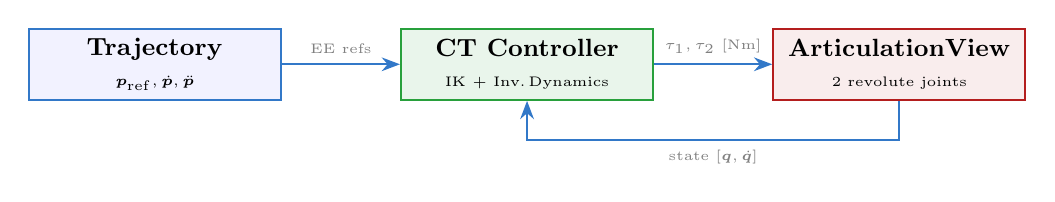
\begin{tikzpicture}[
    node distance=0.6cm and 1.8cm,
    block/.style={rectangle, draw=isaacblue, thick, fill=blue!5,
                  minimum height=0.9cm, minimum width=3.2cm, align=center, font=\small},
    arr/.style={-Stealth, thick, isaacblue},
    port/.style={font=\tiny, text=gray},
]
    \node[block] (ref)  {\textbf{Trajectory}\\{\tiny $\bm{p}_{\mathrm{ref}}, \dot{\bm{p}}, \ddot{\bm{p}}$}};
    \node[block, right=1.5cm of ref, fill=isaacgreen!10, draw=isaacgreen] (ct) {\textbf{CT Controller}\\{\tiny IK + Inv.\,Dynamics}};
    \node[block, right=1.5cm of ct, fill=darkred!8, draw=darkred] (plant) {\textbf{ArticulationView}\\{\tiny 2 revolute joints}};

    \draw[arr] (ref) -- (ct) node[midway, above, port] {EE refs};
    \draw[arr] (ct) -- (plant) node[midway, above, port] {$\tau_1, \tau_2$ [Nm]};
    \draw[arr] (plant.south) -- ++(0,-0.5) -| (ct.south)
        node[pos=0.25, below, port] {state $[\bq, \dot{\bq}]$};
\end{tikzpicture}
\end{center}
\end{archbox}

\subsection{Algorithm Flow --- Step by Step}

Every simulation step the controller executes:

\begin{enumerate}[leftmargin=2em]
    \item \textbf{Read state} $(\bq, \dot{\bq})$ from \texttt{ArticulationView.get\_joint\_positions / velocities}
    \item \textbf{Evaluate trajectory} $\to$ desired EE position $\bm{p}_{\mathrm{ref}}$, velocity $\dot{\bm{p}}_{\mathrm{ref}}$, acceleration $\ddot{\bm{p}}_{\mathrm{ref}}$
    \item \textbf{Inverse kinematics}: $\bm{p}_{\mathrm{ref}} \xrightarrow{\text{2R analytical}} \bq_{\mathrm{des}}$
    \item \textbf{Differential IK}: $\dot{\bm{p}}_{\mathrm{ref}} \xrightarrow{\bJ^{-1}} \dot{\bq}_{\mathrm{ref}}$, \quad $\ddot{\bm{p}}_{\mathrm{ref}} \xrightarrow{\bJ^{-1}} \ddot{\bq}_{\mathrm{ref}}$
    \item \textbf{PD + feedforward}: $\bm{a}_{\mathrm{des}} = \ddot{\bq}_{\mathrm{ref}} + K_p(\bq_{\mathrm{des}} - \bq) + K_d(\dot{\bq}_{\mathrm{ref}} - \dot{\bq})$
    \item \textbf{Inverse dynamics}: $\btau = \bM(\bq)\,\bm{a}_{\mathrm{des}} + \bh(\bq, \dot{\bq})$ \quad via PhysX tensor API
    \item \textbf{Saturate and apply}: $\btau_{\mathrm{clip}} = \mathrm{clip}(\btau, \pm\tau_{\max})$ $\to$ \texttt{set\_joint\_efforts()}
\end{enumerate}

\subsection{What the Cable Is (and Isn't)}

\begin{warnbox}
\textbf{The cable/belt is NOT modeled as a physical element.}  The PhysX articulation contains only two rigid revolute joints---there is no spring, cable, or pulley in the physics simulation.  The belt is treated as a \textbf{rigid tendon}: an inextensible, massless transmission between motor and joint.
\end{warnbox}

The controller writes \textbf{joint torques} $[\tau_1, \tau_2]$ in Nm directly via \texttt{set\_joint\_efforts()}.  There is no cable compliance, no pulley friction, and no belt elasticity in the dynamics.

Cable tensions are a \textbf{post-hoc decomposition} for logging:
\[
    F_{\mathrm{net}} = \frac{\tau_2}{r_p}, \qquad
    T_{\mathrm{green}} = \max(F_{\mathrm{net}}, 0), \qquad
    T_{\mathrm{red}} = \max(-F_{\mathrm{net}}, 0)
\]
These appear in the log arrays and plots but are never fed back into PhysX.  The cable visualization (coloured polylines in the Isaac Sim viewport) is likewise computed from FK for rendering only.

\newpage

% ============================================================================
\section{Motivation: From PyDrake to Isaac Sim}
\label{sec:motivation}
% ============================================================================

The PyDrake implementation (see companion document) validates the computed-torque controller with analytical dynamics and Meshcat visualization. \textbf{This Isaac Sim version} re-implements the same control law using NVIDIA's physics stack for two reasons:

\begin{enumerate}[leftmargin=2em]
    \item \textbf{GPU acceleration}: PhysX runs natively on CUDA, enabling future RL training with thousands of parallel environments.
    \item \textbf{Isaac Lab compatibility}: The same \texttt{ArticulationView} API used here is used by IsaacLab for GPU-parallel simulation.
\end{enumerate}

\begin{archbox}{Key Architectural Difference}
\begin{center}
\begin{tabular}{lcc}
\toprule
\textbf{Component} & \textbf{PyDrake Version} & \textbf{Isaac Sim Version} \\
\midrule
Physics engine & Drake MultibodyPlant & NVIDIA PhysX 5 \\
$\bM(\bq)$ source & \texttt{CalcMassMatrix()} & \texttt{ArticulationView} tensor \\
$\bh(\bq,\bdq)$ source & \texttt{CalcBiasTerm()} & \texttt{get\_coriolis\_and\_centrifugal()} \\
 & & $+$ \texttt{get\_generalized\_gravity()} \\
Controller & Drake \texttt{LeafSystem} & Pure NumPy function \\
Visualization & Meshcat (browser) & Isaac Sim native viewport / USD \\
IK solver & Drake \texttt{InverseKinematics} & Pure NumPy 2R closed-form \\
Trajectory & \texttt{PiecewisePolynomial} & \texttt{scipy.CubicSpline} \\
\bottomrule
\end{tabular}
\end{center}
\end{archbox}


% ============================================================================
\section{System Architecture}
\label{sec:architecture}
% ============================================================================

\subsection{High-Level Pipeline}

\begin{archbox}{Isaac Sim CT Controller Pipeline}
\begin{center}
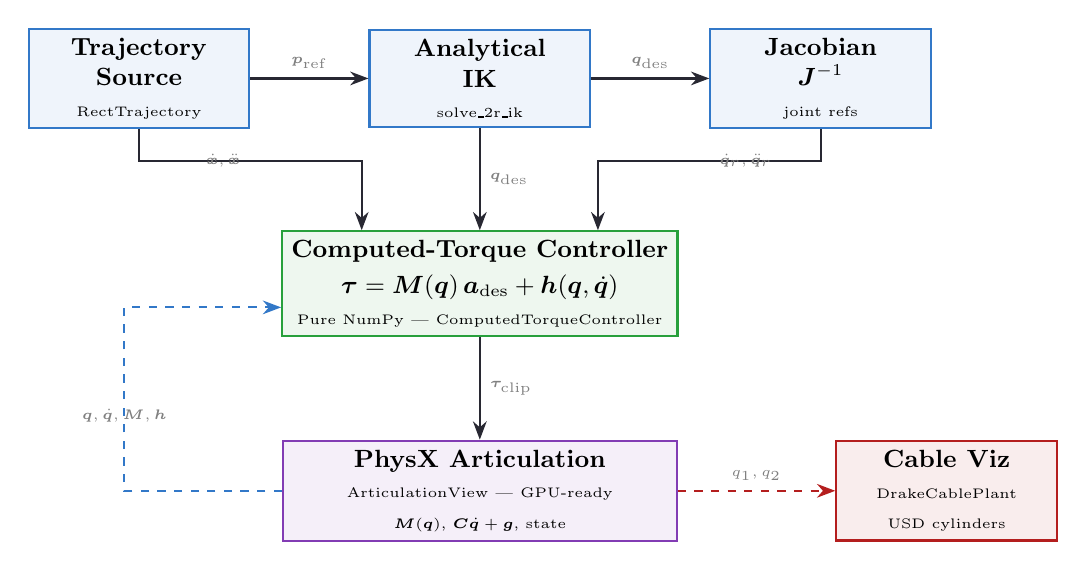
\begin{tikzpicture}[
    node distance=0.8cm and 1.5cm,
    block/.style={rectangle, draw=#1, thick, fill=#1!8,
                  minimum height=1.0cm, minimum width=2.8cm, align=center, font=\small},
    block/.default=isaacorg,
    port/.style={font=\tiny, text=gray},
    arr/.style={-Stealth, thick, isaacdark},
    data/.style={-Stealth, thick, isaacblue, dashed},
]
    % Row 1: References
    \node[block=isaacblue] (traj) {\textbf{Trajectory}\\\textbf{Source}\\{\tiny RectTrajectory}};
    \node[block=isaacblue, right=1.5cm of traj] (ik) {\textbf{Analytical}\\\textbf{IK}\\{\tiny solve\_2r\_ik}};
    \node[block=isaacblue, right=1.5cm of ik] (jac) {\textbf{Jacobian}\\\textbf{$\bJ^{-1}$}\\{\tiny joint refs}};

    % Row 2: Controller
    \node[block=isaacgreen, below=1.3cm of ik, minimum width=5cm] (ct) {%
        \textbf{Computed-Torque Controller}\\[2pt]
        {\small $\btau = \bM(\bq)\,\bm{a}_{\mathrm{des}} + \bh(\bq, \bdq)$}\\
        {\tiny Pure NumPy --- ComputedTorqueController}};

    % Row 3: Physics
    \node[block=physxpurple, below=1.3cm of ct, minimum width=5cm] (phys) {%
        \textbf{PhysX Articulation}\\
        {\tiny ArticulationView --- GPU-ready}\\
        {\tiny $\bM(\bq)$, $\bm{C}\bdq + \bm{g}$, state}};

    % Side: Cable Viz
    \node[block=darkred, right=2.0cm of phys] (cable) {%
        \textbf{Cable Viz}\\
        {\tiny DrakeCablePlant}\\
        {\tiny USD cylinders}};

    % Connections
    \draw[arr] (traj) -- (ik) node[midway, above, port] {$\bm{p}_{\mathrm{ref}}$};
    \draw[arr] (ik) -- (jac) node[midway, above, port] {$\bq_{\mathrm{des}}$};
    \draw[arr] (traj.south) -- ++(0,-0.4) -| ([xshift=-1.5cm]ct.north) node[pos=0.25, left, port] {$\dot{\bx}, \ddot{\bx}$};
    \draw[arr] (jac.south) -- ++(0,-0.4) -| ([xshift=1.5cm]ct.north) node[pos=0.25, right, port] {$\bdq_r, \bddq_r$};
    \draw[arr] (ik.south) -- (ct.north) node[pos=0.5, right, port] {$\bq_{\mathrm{des}}$};

    \draw[arr] (ct) -- (phys) node[midway, right, port] {$\btau_{\mathrm{clip}}$};

    % Feedback
    \draw[data] (phys.west) -- ++(-2.0, 0) |- ([yshift=-0.3cm]ct.west)
        node[pos=0.25, below, port] {$\bq, \bdq, \bM, \bh$};

    % Cable
    \draw[data, darkred] (phys.east) -- (cable.west) node[midway, above, port] {$q_1, q_2$};
\end{tikzpicture}
\end{center}
\end{archbox}

\subsection{Import Order --- Critical Rule}

\begin{warnbox}
Isaac Sim requires \texttt{SimulationApp} to be instantiated \textbf{before any other \texttt{omni.*} or \texttt{isaacsim.*} import}. Violating this crashes Python without a useful error message.
\end{warnbox}

\subsubsection*{Quiet startup via \texttt{IsaacSimLogger}}

Isaac Sim writes $\sim$500 lines of kit/carb noise (extension loading, GPU bandwidth tables, deprecation warnings) to file descriptors 1 and 2 \textbf{from C++}, bypassing \texttt{sys.stdout}. The \texttt{IsaacSimLogger} uses \texttt{os.dup2} to redirect fds at the OS level:

\begin{lstlisting}[caption={\texttt{project\_utils/log\_isaacsim.py} --- key methods}]
class IsaacSimLogger:
    @classmethod
    def from_argv(cls) -> "IsaacSimLogger":
        """Verbose mode if --verbose in sys.argv, else quiet."""
        return cls(verbose=("--verbose" in sys.argv))

    def suppress(self):
        """Redirect fds 1+2 to /dev/null (OS-level, bypasses C++)."""
        if self._verbose: return
        self._saved1 = os.dup(1);  self._saved2 = os.dup(2)
        devnull = os.open(os.devnull, os.O_WRONLY)
        os.dup2(devnull, 1);  os.dup2(devnull, 2)
        os.environ["CARB_LOG_LEVEL"] = "error"
        atexit.register(self._restore_fds)  # crash safety

    def restore(self):
        """Restore fds; print Isaac Sim ready message."""
        if self._verbose: return
        self._restore_fds()
        elapsed = time.time() - self._t0
        print(f"Isaac Sim ready ({elapsed:.1f}s) --- use --verbose for full log")
\end{lstlisting}

\begin{resultbox}
502 lines before / 139 lines after (72\% reduction). Normal Python tracebacks remain fully visible because fds are restored before the custom \texttt{excepthook} fires.
\end{resultbox}

\begin{lstlisting}[caption={Mandatory import sequence --- \texttt{script\_cup\_manipulator\_pendulam\_tendon\_computed\_torque\_isaac\_sim.py}}]
import os, sys
from pathlib import Path

# Project root on sys.path (needed before SimulationApp)
_PROJECT_ROOT = str(Path(__file__).resolve().parent)
if _PROJECT_ROOT not in sys.path:
    sys.path.insert(0, _PROJECT_ROOT)

# Pre-parse --render (cannot use argparse yet)
_RENDER_CHOICES = ("native", "websocket", "headless")
_render_mode = "native"
for _i, _arg in enumerate(sys.argv):
    if _arg == "--render" and _i + 1 < len(sys.argv):
        _render_mode = sys.argv[_i + 1]
        if _render_mode not in _RENDER_CHOICES:
            print(f"[ERROR] --render must be one of {_RENDER_CHOICES}")
            sys.exit(1)

# QUIET mode: suppress Isaac Sim extension/GPU/warning noise at startup.
# Use --verbose to restore original output.
from project_utils.log_isaacsim import IsaacSimLogger
_log = IsaacSimLogger.from_argv()  # no-op when --verbose in sys.argv
_log.suppress()

import warnings
warnings.filterwarnings("ignore", category=DeprecationWarning)

# FIRST Isaac Sim import
from isaacsim import SimulationApp
simulation_app = SimulationApp({
    "headless": _render_mode != "native",  # native -> local window
    "width": 1280, "height": 720,
    "hide_ui": True,
})

# NOW safe to import Isaac Sim modules
from omni.isaac.core import World
from omni.isaac.core.articulations import ArticulationView

# WebRTC streaming (--render websocket) -- set up BEFORE world init
if _render_mode == "websocket":
    import subprocess
    from omni.kit.livestream.webrtc import set_setting, enable_extension
    try:
        _ip = subprocess.check_output(
            ["tailscale", "ip", "-4"], text=True).strip()
    except Exception:
        _ip = "127.0.0.1"  # fallback: localhost
    set_setting("/app/livestream/publicEndpointAddress", _ip)
    enable_extension("omni.kit.livestream.webrtc")
    _log.print(f"  WebRTC (Tailscale) : connect to  {_ip} : 49100")

# Startup complete -- restore stdout/stderr
_log.restore()
\end{lstlisting}

\begin{resultbox}
\textbf{WebRTC streaming to Mac / tablet via Tailscale}:
\begin{enumerate}[leftmargin=2em, itemsep=2pt]
    \item Install Tailscale on both machines and join the same tailnet.
    \item Start with \texttt{--render websocket}.
    \item Open the Isaac Sim WebRTC Streaming Client on the Mac; connect to the printed Tailscale IP on port 49100.
\end{enumerate}
Critical: \texttt{set\_setting("/app/livestream/publicEndpointAddress", ip)} must point to the Tailscale IP, not the LAN IP, for ICE negotiation to succeed across the VPN.  Without it the Mac client receives an unreachable address and the stream never opens.
\end{resultbox}


% ============================================================================
\section{Dynamics via PhysX ArticulationView}
\label{sec:dynamics}
% ============================================================================

\subsection{Manipulator Equation of Motion (Review)}

The same rigid-body dynamics apply regardless of the physics engine:

\begin{equation}
\boxed{
\bM(\bq)\,\bddq + \underbrace{\bm{C}(\bq, \bdq)\,\bdq + \bm{g}(\bq)}_{\bh(\bq, \bdq)} = \btau
}
\label{eq:eom}
\end{equation}

\noindent where:
\begin{itemize}[leftmargin=2em]
    \item $\bM(\bq) \in \mathbb{R}^{2\times 2}$ --- mass (inertia) matrix
    \item $\bm{C}(\bq, \bdq)\,\bdq \in \mathbb{R}^2$ --- Coriolis and centrifugal forces
    \item $\bm{g}(\bq) \in \mathbb{R}^2$ --- gravitational torques
    \item $\bh(\bq, \bdq) = \bm{C}\bdq + \bm{g}$ --- bias vector
\end{itemize}

\subsection{PhysX Tensor API --- Dynamics Queries}

Isaac Sim exposes these quantities through the \texttt{ArticulationView} in a GPU-tensor-compatible format:

\begin{lstlisting}[caption={Dynamics initialization --- \texttt{robots/cup\_manipulator\_tendon\_isaac.py}}]
class CupManipulatorTendonIsaac:
    def initialize_dynamics_view(self, world):
        """Create ArticulationView for dynamics (M, C, g) queries."""
        self._art_view = ArticulationView(
            prim_paths_expr="/World/manipulator_cable",
            name="manip_dynamics",
        )
        world.scene.add(self._art_view)
        self._art_view.initialize(world.physics_sim_view)
\end{lstlisting}

\begin{lstlisting}[caption={Mass matrix and bias forces --- \texttt{robots/cup\_manipulator\_tendon\_isaac.py}}]
def get_mass_matrix(self):
    """Return (2,2) mass matrix for actuated DOFs."""
    M_full = self._art_view.get_mass_matrices()  # (1, n_dof, n_dof)
    M = M_full[0]  # single environment
    idx = self._actuated_dof_indices
    return M[np.ix_(idx, idx)]  # extract actuated 2x2 block

def get_coriolis_and_centrifugal(self):
    """Return (2,) Coriolis+centrifugal forces."""
    return self._art_view.get_coriolis_and_centrifugal_forces()[0][
        self._actuated_dof_indices]

def get_generalized_gravity(self):
    """Return (2,) gravity torques."""
    return self._art_view.get_generalized_gravity_forces()[0][
        self._actuated_dof_indices]

def get_bias_forces(self):
    """h(q, q_dot) = C(q,q_dot)q_dot + g(q)"""
    return self.get_coriolis_and_centrifugal() \
         + self.get_generalized_gravity()
\end{lstlisting}

\begin{codemath}
The three PhysX tensor calls map directly to the terms in \eqref{eq:eom}:

\begin{tabular}{lll}
\texttt{get\_mass\_matrices()} & $\to$ & $\bM(\bq) \in \mathbb{R}^{2\times 2}$ \\
\texttt{get\_coriolis\_and\_centrifugal\_forces()} & $\to$ & $\bm{C}(\bq,\bdq)\,\bdq \in \mathbb{R}^2$ \\
\texttt{get\_generalized\_gravity\_forces()} & $\to$ & $\bm{g}(\bq) \in \mathbb{R}^2$ \\
\end{tabular}

\medskip
The bias vector is their sum: $\bh = \bm{C}\bdq + \bm{g}$.

\textbf{Index mapping}: The URDF may contain passive/fixed joints. The \texttt{\_actuated\_dof\_indices} array selects only the two revolute DOFs $[q_1, q_2]$ from the full articulation state.
\end{codemath}

\subsection{PhysX Drive Configuration --- Critical Fix}

\begin{physxbox}{PhysX Drive Stiffness Bug --- Root Cause of Initial Failure}
When loading a URDF, Isaac Sim maps the \texttt{<limit effort="10"/>} attribute to the PhysX \texttt{angular drive}'s \texttt{maxForce=10}. Furthermore, PhysX drives default to a non-zero \texttt{stiffness}, creating a \textbf{position spring} that fights the effort commands.

For pure effort (torque) control, both must be overridden:
\[
    \texttt{stiffness} = 0, \qquad \texttt{maxForce} = 10^4 \;\text{Nm}
\]
Otherwise the 5.3\,kg arm's gravity ($\approx 10$\,Nm) consumes the entire effort budget.
\end{physxbox}

\begin{lstlisting}[caption={PhysX drive fix --- \texttt{robots/cup\_manipulator\_tendon\_isaac.py}}]
def add_joint_actuators(self):
    """Configure PhysX angular drives for pure effort control."""
    for jt_name in [self.JT1_NAME, self.JT2_NAME]:
        drive = UsdPhysics.DriveAPI.Get(joint_prim, "angular")
        # CRITICAL: zero stiffness (no position spring)
        drive.GetStiffnessAttr().Set(0.0)
        # CRITICAL: high maxForce (override URDF effort="10")
        drive.GetMaxForceAttr().Set(1e4)
        # Damping from config (viscous friction model)
        drive.GetDampingAttr().Set(float(jt_cfg.damping))
\end{lstlisting}

\begin{codemath}
PhysX applies the drive force as:
\[
    \tau_{\mathrm{PhysX}} = \underbrace{k_s \cdot (q_{\mathrm{target}} - q)}_{\text{spring (must be 0)}}
    + \underbrace{k_d \cdot (\dot q_{\mathrm{target}} - \dot q)}_{\text{damping}}
    + \underbrace{\tau_{\mathrm{effort}}}_{\text{our command}}
\]
Clamped to $[-\texttt{maxForce},\; +\texttt{maxForce}]$. Setting $k_s = 0$ and $\texttt{maxForce} = 10^4$ ensures our computed-torque command $\btau$ passes through to the articulation without interference.
\end{codemath}


% ============================================================================
\section{Computed-Torque Controller --- Pure NumPy}
\label{sec:ct}
% ============================================================================

\subsection{Control Law}

Identical to the PyDrake version (Section~\ref{sec:ct_law_eq} below), but using NumPy arrays instead of Drake \texttt{LeafSystem} callbacks:

\begin{equation}
\boxed{
\bm{a}_{\mathrm{des}} = \bddq_{\mathrm{ref}} + K_p\,(\bq_{\mathrm{des}} - \bq) + K_d\,(\bdq_{\mathrm{ref}} - \bdq)
}
\label{sec:ct_law_eq}
\end{equation}

\begin{equation}
\boxed{
\btau = \bM(\bq)\,\bm{a}_{\mathrm{des}} + \bh(\bq, \bdq)
}
\label{eq:ct_isaac}
\end{equation}

The closed-loop error dynamics are:

\begin{equation}
    \ddot{\bm{e}} + K_d\,\dot{\bm{e}} + K_p\,\bm{e} = \bm{0}
    \qquad \Longrightarrow \qquad
    \omega_n = \sqrt{K_p},\; \zeta = \frac{K_d}{2\sqrt{K_p}}
\end{equation}

\begin{resultbox}
For $K_p = 800$, $K_d = 40$: $\omega_n \approx 28.3$\,rad/s, $\zeta \approx 0.71$ (underdamped). At $\Delta t = 10$\,ms (100\,Hz), the Nyquist frequency is $\pi/\Delta t \approx 314$\,rad/s, giving a ratio $\omega_n / \omega_{\mathrm{Nyq}} \approx 0.09$ --- well within the safe sampling margin.
\end{resultbox}

\subsection{Controller Implementation}

\begin{lstlisting}[caption={Engine-agnostic CT controller --- \texttt{controller/computed\_torque\_isaacsim.py}}]
class ComputedTorqueController:
    def __init__(self, Kp=800.0, Kd=40.0, tau_max=50.0,
                 pulley_radius=60*0.005/(2*np.pi)):
        self.Kp = float(Kp)
        self.Kd = float(Kd)
        self.tau_max = float(tau_max)
        self.r_p = float(pulley_radius)

    def compute(self, q, q_dot, q_des, q_dot_ref, q_ddot_ref, M, h):
        # PD + feedforward acceleration
        a_des = q_ddot_ref + self.Kp * (q_des - q) \
                           + self.Kd * (q_dot_ref - q_dot)
        # Inverse dynamics
        tau_raw = M @ a_des + h
        # Cable tension decomposition (joint 2)
        F_net = tau_raw[1] / self.r_p
        T_green = max(F_net, 0.0)
        T_red   = max(-F_net, 0.0)
        tau2_cmd = (T_green - T_red) * self.r_p
        # Clip
        tau_clip = np.clip(
            np.array([tau_raw[0], tau2_cmd]),
            -self.tau_max, self.tau_max)
        return CTControllerOutput(tau_clip=tau_clip, ...)
\end{lstlisting}

\begin{codemath}
The controller is \textbf{identical} to the PyDrake version --- only the \emph{source} of $\bM$ and $\bh$ changes:
\begin{itemize}
    \item \textbf{PyDrake}: \texttt{plant.CalcMassMatrix(context)}, \texttt{plant.CalcBiasTerm(context)}
    \item \textbf{Isaac Sim}: \texttt{art\_view.get\_mass\_matrices()}, \texttt{get\_coriolis+gravity}
\end{itemize}

Cable tension decomposition:
\[
    F_{\mathrm{net}} = \frac{\tau_2}{\rp}, \quad
    T_{\mathrm{green}} = \max(F_{\mathrm{net}}, 0), \quad
    T_{\mathrm{red}} = \max(-F_{\mathrm{net}}, 0)
\]
\[
    \tau_{2,\mathrm{cmd}} = (T_{\mathrm{green}} - T_{\mathrm{red}}) \cdot \rp, \qquad
    \btau_{\mathrm{clip}} = \mathrm{clip}(\btau, -\tau_{\max}, +\tau_{\max})
\]
\end{codemath}

\subsection{IK and Differential IK --- NumPy Only}

\begin{lstlisting}[caption={IK-to-joint-space pipeline --- \texttt{controller/computed\_torque\_isaacsim.py}}]
def ik_to_joint_space_references(
    ee_pos_ref, ee_vel_ref, ee_acc_ref,
    L1, L2, q_seed, solve_ik_fn):
    """EE refs -> joint-space (q_des, q_dot_ref, q_ddot_ref)."""
    q_des, ok = solve_ik_fn(L1, L2, ee_pos_ref, q_seed)
    # Analytical Jacobian at q_des
    q1d, q2d = q_des
    s1, c1 = np.sin(q1d), np.cos(q1d)
    s12, c12 = np.sin(q1d+q2d), np.cos(q1d+q2d)
    J = np.array([
        [-L1*s1 - L2*s12, -L2*s12],
        [ L1*c1 + L2*c12,  L2*c12]])
    J_inv = np.linalg.pinv(J)
    q_dot_ref  = J_inv @ ee_vel_ref
    q_ddot_ref = J_inv @ ee_acc_ref
    return q_des, q_dot_ref, q_ddot_ref, ok
\end{lstlisting}

\begin{codemath}
\textbf{Step 1 --- Position IK} (closed-form 2R):
\[
    \cos q_2 = \frac{x^2 + y^2 - L_1^2 - L_2^2}{2L_1 L_2}, \quad
    q_1 = \text{atan2}(y, x) - \text{atan2}(L_2 s_2,\; L_1 + L_2 c_2)
\]

\textbf{Step 2 --- Velocity mapping} via Jacobian:
\[
    \bdq_{\mathrm{ref}} = \bJ^{-1}(\bq_{\mathrm{des}})\,\dot{\bx}_{\mathrm{ref}}
\]

\textbf{Step 3 --- Acceleration mapping} (simplified, drops $\dot{\bJ}\bdq$ bias):
\[
    \bddq_{\mathrm{ref}} \approx \bJ^{-1}(\bq_{\mathrm{des}})\,\ddot{\bx}_{\mathrm{ref}}
\]
\end{codemath}


% ============================================================================
\section{Trajectory Generation}
\label{sec:traj}
% ============================================================================

\subsection{Pure SciPy Trajectories (No Drake)}

The Isaac Sim version uses \texttt{scipy.interpolate.CubicSpline} with periodic boundary conditions to create $C^2$ trajectories:

\begin{lstlisting}[caption={Looping cubic spline --- \texttt{controller/trajectory.py}}]
class LoopingCubicTrajectory:
    def __init__(self, t_breaks, waypoints, period):
        self.period = period
        self._cs = CubicSpline(t_breaks, waypoints, bc_type='periodic')
        self._cs_vel = self._cs.derivative(1)
        self._cs_acc = self._cs.derivative(2)

    def eval_position(self, t):
        return self._cs(t % self.period)

    def eval_velocity(self, t):
        return self._cs_vel(t % self.period)

    def eval_acceleration(self, t):
        return self._cs_acc(t % self.period)
\end{lstlisting}

\begin{codemath}
Periodic cubic spline satisfies at the wrap boundary:
\[
    \bm{p}(0) = \bm{p}(T), \quad
    \dot{\bm{p}}(0) = \dot{\bm{p}}(T), \quad
    \ddot{\bm{p}}(0) = \ddot{\bm{p}}(T) \qquad (C^2 \text{ continuity})
\]
The time modulus $t \mapsto t \bmod T$ produces an infinite looping trajectory from a single lap.
\end{codemath}

\subsection{Rectangle --- Velocity Profiling}

The rectangle uses \textbf{non-uniform time stamps} for velocity profiling (slow at corners, fast on straights):

\begin{equation}
    v(s) = v_{\mathrm{corner}} + (v_{\mathrm{max}} - v_{\mathrm{corner}}) \cdot h\!\left(\frac{d(s)}{d_{\mathrm{blend}}}\right),
    \qquad h(t) = t^2(3 - 2t)
\end{equation}

where $d(s)$ is the arc-length distance to the nearest corner and $h(t)$ is the Hermite smoothstep interpolant.

\subsection{Move-to-Start --- Cubic Hermite Preamble}

Before tracking begins, a \textbf{cubic Hermite spline} moves the arm from rest to the first waypoint:

\begin{lstlisting}[caption={Preamble construction --- \texttt{controller/trajectory.py}}]
class PreambleTrajectorySource:
    """During t < move_duration: approach spline.
       After: main looping trajectory."""
    def eval_position(self, t):
        if self._move is not None and t < self.move_duration:
            return self._move.eval_position(t)
        return self._main.eval_position(t - self.move_duration)
\end{lstlisting}

Boundary conditions:
\begin{equation}
    \bm{p}(0) = \bm{p}_{\mathrm{home}}, \quad
    \dot{\bm{p}}(0) = \bm{0}, \quad
    \bm{p}(T_m) = \bm{p}_{\mathrm{traj}}(0), \quad
    \dot{\bm{p}}(T_m) = \dot{\bm{p}}_{\mathrm{traj}}(0)
\end{equation}


% ============================================================================
\section{Simulation Loop --- Step by Step}
\label{sec:loop}
% ============================================================================

\subsection{Setup Phase}

\begin{lstlisting}[caption={World and robot setup --- \texttt{script\_cup\_manipulator\_pendulam\_tendon\_computed\_torque\_isaac\_sim.py}}]
# 1. Create robot wrapper
manip = CupManipulatorTendonIsaac(MANIP_CONFIG)
manip.prepare_usd()           # Convert URDF -> USD

# 2. Create World
world = World(
    stage_units_in_meters=1.0,
    physics_dt=args.dt,       # 10 ms
    rendering_dt=args.dt,
)
world.scene.add_default_ground_plane()

# 3. Load robot
manip.load_urdf(world)
manip.weld_base_to_world(position=np.zeros(3), orientation=orient)
manip.add_end_effector_frame()
manip.set_joint_properties()
manip.add_joint_actuators()   # stiffness=0, maxForce=1e4

# 4. Cable viz -- prims BEFORE world.reset()
cable_viz = CableVisualizerIsaac(stage, drake_urdf)
cable_viz.create_prims(q1=q1_init, q2=q2_init)

# 5. Reset and initialize
world.reset()
manip.initialize_state()
manip.initialize_dynamics_view(world)
\end{lstlisting}

\begin{warnbox}
The cable USD cylinder prims must be created \textbf{before} \texttt{world.reset()} to avoid invalidating the \texttt{ArticulationView}. Adding/removing prims after reset triggers a PhysX topology change that crashes \texttt{physics\_sim\_view}.
\end{warnbox}

\subsection{Control Loop}

\begin{lstlisting}[caption={Main simulation loop.}]
while not stop_requested and step < max_steps:
    # 1. Read current state from PhysX
    q     = manip.get_positions_user_order()    # [q1, q2]
    q_dot = manip.get_velocities_user_order()   # [dq1, dq2]

    # 2. Evaluate trajectory at current time
    ee_pos_ref = traj_source.eval_position(t)
    ee_vel_ref = traj_source.eval_velocity(t)
    ee_acc_ref = traj_source.eval_acceleration(t)

    # 3. IK + Jacobian -> joint-space references
    q_des, q_dot_ref, q_ddot_ref, ik_ok = \
        ik_to_joint_space_references(
            ee_pos_ref, ee_vel_ref, ee_acc_ref,
            L1, L2, last_q_des, solve_2r_ik)
    if ik_ok:
        last_q_des = q_des.copy()     # warm-start seed

    # 4. Dynamics queries from PhysX
    M = manip.get_mass_matrix()        # (2,2)
    h = manip.get_bias_forces()        # (2,)

    # 5. Computed torque
    ct_out = ct.compute(q, q_dot, q_des, q_dot_ref,
                        q_ddot_ref, M, h)

    # 6. Apply torques to articulation
    manip.set_joint_torques(ct_out.tau_clip)

    # 7. Update cable visualization (every N steps)
    if step % _CABLE_UPDATE_INTERVAL == 0:
        cable_viz.update(q[0], q[1])

    # 8. Step physics
    # render=True for native window and websocket stream; False only for headless
    world.step(render=(_render_mode != "headless"))
    t += args.dt;  step += 1
\end{lstlisting}

\begin{warnbox}
\textbf{WebRTC streaming requires \texttt{render=True}.} Setting \texttt{render=False} skips the viewport update, so the Mac client receives no frames. The correct predicate is \texttt{render=(\_render\_mode != "headless")} --- not \texttt{== "native"}.
\end{warnbox}

\begin{codemath}
Each iteration of the loop executes the full CT pipeline:

\textbf{(1) State read}: $[\bq, \bdq] \leftarrow$ \texttt{ArticulationView}

\textbf{(2) Reference}: $[\bm{p}_r(t), \dot{\bm{p}}_r(t), \ddot{\bm{p}}_r(t)] \leftarrow$ cubic spline

\textbf{(3) IK}: $\bm{p}_r \xrightarrow{\text{2R}} \bq_d$, \quad $\dot{\bm{p}}_r \xrightarrow{\bJ^{-1}} \bdq_r$, \quad $\ddot{\bm{p}}_r \xrightarrow{\bJ^{-1}} \bddq_r$

\textbf{(4) Dynamics}: $\bM(\bq), \bh(\bq,\bdq) \leftarrow$ PhysX tensors

\textbf{(5) Control}: $\bm{a}_d = \bddq_r + K_p(\bq_d - \bq) + K_d(\bdq_r - \bdq)$, \; $\btau = \bM\,\bm{a}_d + \bh$

\textbf{(6) Apply}: $\btau_{\mathrm{clip}} \to$ PhysX drive effort

\textbf{(7) Cable viz}: Update USD cylinder transforms (every 5 steps for performance)

\textbf{(8) Physics step}: PhysX integrates one $\Delta t$
\end{codemath}


% ============================================================================
\section{Cable Visualization}
\label{sec:cable_viz}
% ============================================================================

\subsection{DrakeCablePlant --- Headless Geometry Engine}

Cable routing geometry cannot be computed purely from PhysX (it has no cable model). Instead, we use a \textbf{headless Drake plant} solely for cable FK:

\begin{lstlisting}[caption={Cable visualization wrapper --- \texttt{project\_utils/viz\_cables\_isaacsim.py}}]
class CableVisualizerIsaac:
    def __init__(self, stage, drake_urdf):
        self._stage = stage
        self._drake = DrakeCablePlant(drake_urdf, 0.0, 0.0)
        self._prim_paths = {}

    def create_prims(self, q1, q2):
        """Pre-allocate USD cylinders at initial pose."""
        self._drake.update(q1, q2)
        self._draw_cables_usd(self._stage, self._drake)

    def update(self, q1, q2):
        """Recompute cable routing and update USD transforms."""
        self._drake.update(q1, q2)
        # Update existing prim positions (no create/delete)
        for route, pts in self._drake.get_cable_world_points():
            for i in range(len(pts) - 1):
                _update_cylinder_prim(
                    self._prim_paths[key],
                    pts[i], pts[i+1])
\end{lstlisting}

\begin{warnbox}
This cable visualization is \textbf{NOT suitable for parallel RL training} --- it runs a CPU-bound Drake plant and modifies the USD stage directly. For RL with $>1$ environment, cable visualization should be replaced with a GPU-native approach or disabled entirely.
\end{warnbox}


% ============================================================================
\section{URDF-to-USD Pipeline}
\label{sec:urdf_usd}
% ============================================================================

\subsection{Conversion Flow}

Isaac Sim requires USD format. The URDF must be converted:

\begin{center}
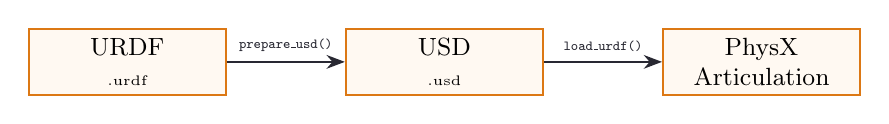
\begin{tikzpicture}[
    node distance=1.5cm,
    block/.style={rectangle, draw=isaacorg, thick, fill=orange!5,
                  minimum height=0.7cm, minimum width=2.5cm, align=center, font=\small},
    arr/.style={-Stealth, thick, isaacdark},
]
    \node[block] (urdf) {URDF\\{\tiny .urdf}};
    \node[block, right=of urdf] (usd) {USD\\{\tiny .usd}};
    \node[block, right=of usd] (phyx) {PhysX\\Articulation};

    \draw[arr] (urdf) -- (usd) node[midway, above, font=\tiny] {\texttt{prepare\_usd()}};
    \draw[arr] (usd) -- (phyx) node[midway, above, font=\tiny] {\texttt{load\_urdf()}};
\end{tikzpicture}
\end{center}

\begin{lstlisting}[caption={URDF to USD conversion --- \texttt{robots/cup\_manipulator\_tendon\_isaac.py}}]
def prepare_usd(self):
    """Convert URDF -> USD (BEFORE World creation)."""
    import omni.kit.commands
    result, prim_path = omni.kit.commands.execute(
        "URDFParseAndImportFile",
        urdf_path=self.config.urdf_path,
        dest_path="/World/manipulator_cable",
    )

def load_urdf(self, world):
    """After USD is on stage, configure articulation."""
    self.apply_urdf_colors()  # Map <material> -> USD
\end{lstlisting}

\subsection{Color Mapping from URDF}

The URDF \texttt{<material><color>} tags are translated to USD material sublayers via \texttt{apply\_urdf\_colors()}, preserving the visual appearance from the CAD model.


% ============================================================================
\section{Torque Application}
\label{sec:torque_apply}
% ============================================================================

\begin{lstlisting}[caption={Applying torques to PhysX --- \texttt{robots/cup\_manipulator\_tendon\_isaac.py}}]
def set_joint_torques(self, torques):
    """Apply [tau1, tau2] to articulation via ArticulationView."""
    effort = np.zeros(self._art_view.num_dof)
    for i, idx in enumerate(self._actuated_dof_indices):
        effort[idx] = float(torques[i])
    self._art_view.set_joint_efforts(
        effort.reshape(1, -1))  # (1, n_dof) for 1 env
\end{lstlisting}

\begin{codemath}
The effort is injected into the PhysX solver as a generalized force. With the drive configured as:
\[
    k_s = 0 \text{ (no spring)}, \qquad \texttt{maxForce} = 10^4 \text{ Nm}
\]
the effective torque on joint $i$ is:
\[
    \tau_i^{\mathrm{PhysX}} = \mathrm{clip}\!\left(\tau_i^{\mathrm{cmd}} + k_d\,(\dot q_{\mathrm{target}} - \dot q_i),\; -\tau_{\max}^{\mathrm{PhysX}},\; +\tau_{\max}^{\mathrm{PhysX}}\right)
\]
With $k_d$ set to a small viscous damping (0.05\,Nm$\cdot$s/rad), the commanded torque dominates.
\end{codemath}


% ============================================================================
\section{Results and Plotting}
\label{sec:results}
% ============================================================================

\subsection{3$\times$3 Diagnostic Plot}

The \texttt{plot\_results()} function generates the same diagnostic layout as the PyDrake version:

\begin{table}[h]
\centering
\caption{Plot layout.}
\begin{tabular}{lccc}
\toprule
 & \textbf{Position} & \textbf{Velocity} & \textbf{Acceleration} \\
\midrule
\textbf{EE}     & $x, y$ vs ref      & $\dot x, \dot y$ via $\bJ\bdq$ & $\ddot x, \ddot y$ \\
\textbf{Joints}  & $q_1, q_2$ [deg]  & $\dot q_1, \dot q_2$           & $\ddot q_1, \ddot q_2$ \\
\textbf{Forces}  & $\tau$ req vs app  & Cable tensions                 & EE XY path \\
\bottomrule
\end{tabular}
\end{table}

Derived signals:
\begin{itemize}[leftmargin=2em]
    \item EE velocity actual: $\dot{\bm{p}} = \bJ(\bq)\,\bdq$ (exact, no finite differences)
    \item EE acceleration actual: $\ddot{\bm{p}} = \texttt{np.gradient}(\dot{\bm{p}}, t)$
    \item Joint-space references: $\bdq_r = \bJ^{-1}\,\dot{\bx}_r$, $\bddq_r = \bJ^{-1}\,\ddot{\bx}_r$
\end{itemize}

\begin{lstlisting}[caption={FK-based EE actual computation --- \texttt{plot\_results()}}]
# EE actual via FK (no Drake)
ee_x = np.array([forward_kinematics_2r(L1, L2, q[k,0], q[k,1])[0]
                  for k in range(len(t))])
ee_y = np.array([forward_kinematics_2r(L1, L2, q[k,0], q[k,1])[1]
                  for k in range(len(t))])

# EE velocity via Jacobian (analytical, no finite diff)
for k in range(len(t)):
    J = analytical_jacobian_2r(L1, L2, q[k,0], q[k,1])
    v = J @ q_dot[k]
    ee_vx[k], ee_vy[k] = v[0], v[1]
\end{lstlisting}

% Placeholder for figure
\begin{figure}[H]
\centering
\fcolorbox{isaacorg}{orange!3}{%
    \parbox{0.9\textwidth}{\centering\vspace{2cm}
    \textit{Insert Isaac Sim CT results plot here.}\\[0.3cm]
    \texttt{plots/ct\_isaac\_rect\_20260409\_*.png}
    \vspace{2cm}}
}
\caption{Isaac Sim computed-torque tracking results (rectangle). $K_p = 800$, $K_d = 40$, $\tau_{\max} = 50$\,Nm, $\Delta t = 10$\,ms.}
\label{fig:results_isaac}
\end{figure}

\subsection{Performance Metrics}

\begin{resultbox}
\begin{tabular}{ll}
    \textbf{EE tracking RMS} & $\approx 11$\,mm \\
    \textbf{Laps completed} & 4 (in 43\,s wall time for 40\,s sim time) \\
    \textbf{Peak $\tau_1$} & $\approx 15$\,Nm (within 50\,Nm budget) \\
    \textbf{Physics dt} & 10\,ms (100\,Hz) \\
    \textbf{Wall-clock RTF} & $\sim 1\times$ real-time (including render) \\
    \textbf{GPU} & NVIDIA RTX 5090 (31\,GiB) \\
\end{tabular}
\end{resultbox}


% ============================================================================
\section{Running the Simulation}
\label{sec:running}
% ============================================================================

\begin{lstlisting}[language=bash, backgroundcolor=\color{lightgray}, frame=single, rulecolor=\color{gray}]
# Activate Isaac Sim conda environment
conda activate env_isaacsim

# Default: quiet mode, computed-torque, rectangle trajectory, native window
python script_cup_manipulator_pendulam_tendon_computed_torque_isaac_sim.py

# Custom gains and circle trajectory, headless (benchmarking / RL)
python script_cup_manipulator_pendulam_tendon_computed_torque_isaac_sim.py \
    --render headless \
    --ct-kp 800 --ct-kd 40 --ct-tau-max 50 \
    --traj-shape circle --traj-cx 0.4 --traj-radius 0.08 \
    --duration 15

# WebRTC streaming to Mac (Tailscale-routed, port 49100)
python script_cup_manipulator_pendulam_tendon_computed_torque_isaac_sim.py \
    --render websocket
# -> outputs: Mac client: connect to  100.94.173.113 : 49100

# Verbose: restore full Isaac Sim startup log
python script_cup_manipulator_pendulam_tendon_computed_torque_isaac_sim.py \
    --render headless --verbose

# Scene visualization only (no control)
python script_cup_manipulator_pendulam_tendon_scene_viz_isaac_sim.py \
    --render websocket
\end{lstlisting}

\subsubsection*{Render mode summary}

\begin{center}
\begin{tabular}{lll}
\toprule
\textbf{--render} & \textbf{Display} & \textbf{Use case} \\
\midrule
\texttt{native}    & Local OS window  & Development on the GPU machine \\
\texttt{websocket} & WebRTC stream, port 49100 & Remote view from Mac / tablet \\
\texttt{headless}  & None             & Benchmarking, RL training, CI \\
\bottomrule
\end{tabular}
\end{center}


% ============================================================================
\section{Comparison: PyDrake vs Isaac Sim}
\label{sec:comparison}
% ============================================================================

\begin{table}[H]
\centering
\caption{Side-by-side comparison of both implementations.}
\begin{tabular}{p{3.5cm}p{5cm}p{5cm}}
\toprule
\textbf{Aspect} & \textbf{PyDrake} & \textbf{Isaac Sim} \\
\midrule
Physics engine & Drake MultibodyPlant (CPU) & NVIDIA PhysX 5 (GPU-capable) \\
Controller & Drake \texttt{LeafSystem} & Pure NumPy class \\
Signal routing & Drake \texttt{DiagramBuilder} & Manual loop variable passing \\
Mass matrix & \texttt{CalcMassMatrix(ctx)} & \texttt{art\_view.get\_mass\_matrices()} \\
Bias forces & \texttt{CalcBiasTerm(ctx)} & \texttt{get\_coriolis()} + \texttt{get\_gravity()} \\
IK solver & Both: closed-form 2R & Both: closed-form 2R \\
Trajectory & \texttt{PiecewisePolynomial} & \texttt{scipy.CubicSpline} \\
Visualization & Meshcat (browser) & Native viewport or headless \\
Cable viz & Meshcat polylines & USD cylinder prims \\
Timestep & 2\,ms (500\,Hz) & 10\,ms (100\,Hz) \\
RL ready? & No (CPU-only) & Yes (ArticulationView is GPU-parallel) \\
\bottomrule
\end{tabular}
\end{table}


% ============================================================================
\section{Notation Summary}
\label{sec:notation}
% ============================================================================

\begin{table}[h]
\centering
\caption{Notation reference.}
\begin{tabular}{cll}
\toprule
\textbf{Symbol} & \textbf{Description} & \textbf{Unit} \\
\midrule
$\bq = [q_1, q_2]^\top$ & Joint positions & rad \\
$\bdq$ & Joint velocities & rad/s \\
$\bddq$ & Joint accelerations & rad/s$^2$ \\
$\bM(\bq)$ & Mass matrix & kg$\cdot$m$^2$ \\
$\bh(\bq, \bdq)$ & Bias vector $= \bm{C}\bdq + \bm{g}$ & Nm \\
$\btau$ & Applied joint torques & Nm \\
$\bJ(\bq)$ & Analytical Jacobian & m/rad \\
$\bm{p}_{\mathrm{EE}}$ & EE position $[x, y]$ & m \\
$K_p, K_d$ & PD gains & s$^{-2}$, s$^{-1}$ \\
$\omega_n, \zeta$ & Natural frequency, damping ratio & rad/s, --- \\
$\rp$ & Pulley pitch radius & m \\
$T_{\mathrm{green}}, T_{\mathrm{red}}$ & Cable tensions & N \\
$L_1, L_2$ & Link lengths & m \\
$\Delta t$ & Physics timestep & s \\
\bottomrule
\end{tabular}
\end{table}


% ============================================================================
\section{Summary}
% ============================================================================

\begin{archbox}{Implementation Summary}
\begin{enumerate}[leftmargin=2em]
    \item \textbf{No Drake at runtime}: Isaac Sim's \texttt{ArticulationView} provides $\bM(\bq)$ and $\bh(\bq,\bdq)$ via GPU-capable PhysX tensor API
    \item \textbf{Same controller}: Pure-NumPy \texttt{ComputedTorqueController} is engine-agnostic --- shared by both implementations
    \item \textbf{PhysX drive fix}: Setting \texttt{stiffness=0} and \texttt{maxForce=1e4} was critical --- the URDF's \texttt{effort="10"} blocked the entire torque budget
    \item \textbf{Trajectory}: SciPy periodic cubic splines with velocity profiling replace Drake's \texttt{PiecewisePolynomial}
    \item \textbf{Cable viz}: Headless Drake \texttt{CablePlant} drives USD cylinder prims (eval mode only, not for parallel RL)
    \item \textbf{GPU-ready}: The loop structure is compatible with IsaacLab's parallelized \texttt{ArticulationView} for future RL training
\end{enumerate}
\end{archbox}


% ============================================================================
\section{Series Elastic Actuator (SEA) Extension}
\label{sec:sea}
% ============================================================================

The rigid-tendon CT controller (above) assumes $\btau^{\text{applied}} = \btau^{\text{desired}}$.
In the physical system, joint~2 is driven through a compliant cable--spring transmission:

\begin{archbox}{SEA Physical Topology (Joint 2)}
\begin{center}
Motor drum $\;\xrightarrow{\text{cable}}\;$
\textbf{Spring} ($k_s$, $b_c$) $\;\xrightarrow{\text{cable}}\;$
Pulley $\;\to\;$ Link 2
\end{center}
Joint~1 remains rigid direct-drive ($\tau_1^{\text{app}} = \tau_1^{\text{des}}$).
\end{archbox}

\subsection{Motor Rotor Dynamics (Torque Mode)}

The motor model (\texttt{actuators/motor\_dynamics.py}, class \texttt{TorqueMotor})
uses 2nd-order rotor dynamics matching the CubeMars AK60-6 ($N=6$, $\tau_{\text{peak}} = 9\;\text{Nm}$):

\begin{equation}
\boxed{
  J_m \ddot{\theta}_m = \frac{\tau_2^{\text{des}}}{N}
  - b_m\,\dot{\theta}_m - \frac{\rp \cdot F}{N}
}
\end{equation}

Spring extension and cable force:
\begin{align}
  \delta &= \rp \left(\frac{\theta_m}{N} - q_2\right) \\
  F &= k_s \cdot \delta + b_c \cdot \dot{\delta}
\end{align}

Unilateral cable model (cables can only pull):
\[
  T_{\text{green}} = \max(F, 0), \quad T_{\text{red}} = \max(-F, 0), \quad
  \tau_2^{\text{sea}} = \rp \cdot (T_{\text{green}} - T_{\text{red}})
\]

\begin{warnbox}
The SEA creates a first-order lag between $\tau_2^{\text{des}}$ and
$\tau_2^{\text{sea}}$.  For weak springs ($k_s \leq 100\;\text{N/m}$),
this lag causes 20--40\,mm tracking errors on the rectangle trajectory
--- far worse than the $\sim 11\;\text{mm}$ achieved with rigid tendons.
\end{warnbox}

\subsection{SEA Diagnostics}

The \texttt{SEACableActuatorNP.step()} method returns an \texttt{SEADiagnostics}
dataclass with ten fields:

\begin{center}
\begin{tabular}{lll}
\toprule
\textbf{Field} & \textbf{Description} & \textbf{Unit} \\
\midrule
\texttt{motor\_pos}  & $\theta_m / N$ (joint-side) or $l_m$  & rad / m \\
\texttt{motor\_aux}  & $\dot{\theta}_m / N$ or $l_{m,\text{des}}$  & rad/s / m \\
\texttt{delta}       & Spring extension $\delta$              & m \\
\texttt{F\_cable}    & Net cable force                        & N \\
\texttt{tau1\_des}   & Desired $\tau_1$                       & Nm \\
\texttt{tau2\_des}   & Desired $\tau_2$                       & Nm \\
\texttt{T\_green}    & Retracting cable tension               & N \\
\texttt{T\_red}      & Extending cable tension                & N \\
\texttt{tau\_sea}    & Applied $\tau_2$ via spring             & Nm \\
\texttt{tau\_motor}  & Motor-side electromagnetic torque       & Nm \\
\bottomrule
\end{tabular}
\end{center}


% ============================================================================
\section{Residual RL Compensator}
\label{sec:rl}
% ============================================================================

To compensate the SEA lag without hand-tuning a lead compensator, a
residual RL policy is trained on top of the CT controller.

\subsection{Architecture}

\begin{center}
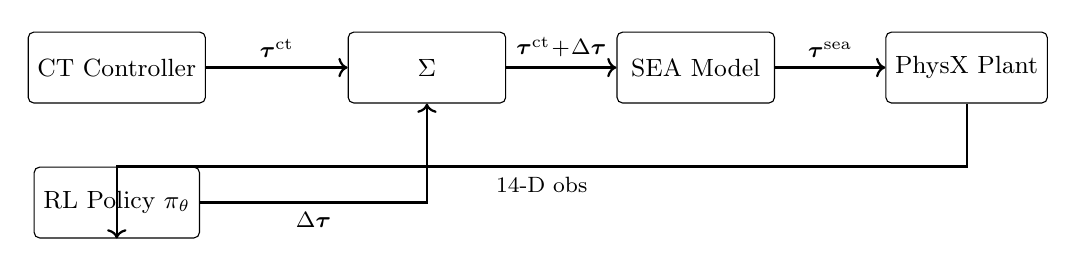
\begin{tikzpicture}[
    block/.style={draw, minimum width=2.0cm, minimum height=0.9cm,
                  rounded corners=2pt, font=\small},
    arr/.style={->, thick},
    node distance=1.6cm and 2.0cm,
]
  \node[block] (ct)   {CT Controller};
  \node[block, below=0.8cm of ct] (rl) {RL Policy $\pi_\theta$};
  \node[block, right=1.8cm of ct] (add) {$\Sigma$};
  \node[block, right=1.4cm of add] (sea) {SEA Model};
  \node[block, right=1.4cm of sea] (plant) {PhysX Plant};

  \draw[arr] (ct.east) -- node[above,font=\footnotesize]{$\btau^{\text{ct}}$} (add.west);
  \draw[arr] (rl.east) -| node[near start,below,font=\footnotesize]{$\Delta\btau$} (add.south);
  \draw[arr] (add.east) -- node[above,font=\footnotesize]{$\btau^{\text{ct}}\!+\!\Delta\btau$} (sea.west);
  \draw[arr] (sea.east) -- node[above,font=\footnotesize]{$\btau^{\text{sea}}$} (plant.west);
  \draw[arr] (plant.south) -- ++(0,-0.8) -| node[near start,below,font=\footnotesize]{14-D obs} (rl.south);
\end{tikzpicture}
\end{center}

The 14-D observation includes joint state, EE error, spring diagnostics
($\delta$, $\dot{\delta}$, $F_{\text{cable}}$), and the CT--SEA torque
mismatch ($\tau_2^{\text{des}} - \tau_2^{\text{app}}$).
The 2-D action $\Delta\btau \in [-5, +5]^2\;\text{Nm}$ is intentionally
small so the RL acts as a \\emph{correction}, not a replacement.

\subsection{What the Policy Learns for Weak Springs}

\begin{resultbox}
The analytical solution (what a perfect policy would learn) is a
\textbf{torque-error I+D compensator}:
\[
  \Delta\btau \approx k_I \int (\btau^{\text{des}} - \btau^{\text{app}})\,dt
  + k_D \frac{d}{dt}(\btau^{\text{des}} - \btau^{\text{app}})
\]
This inverts the first-order spring lag filter.  The RL policy learns this
from data without needing to know $k_s$ explicitly, so it \textbf{generalizes
across spring stiffnesses}.
\end{resultbox}

Specific behaviors for weak springs ($k_s \leq 100\;\text{N/m}$):
\begin{enumerate}[leftmargin=2em]
    \item \textbf{Torque pre-loading}: At trajectory corners, $\Delta\tau_2 > 0$ is sent \emph{before} the corner to pre-charge the spring.
    \item \textbf{Gravity droop correction}: Steady $\Delta\tau_2 < 0$ on downward segments compensates delayed gravity response.
    \item \textbf{Active damping}: During spring oscillations, the residual is $180^\circ$ out of phase.
    \item \textbf{Cross-joint coupling}: $\Delta\tau_1$ corrects Coriolis errors caused by joint-2's delayed spring response.
\end{enumerate}

See the companion RL notes (\texttt{rl/notes/residual\_rl\_implementation.tex})
for the full reward function, PPO hyperparameters, and training details.


% ============================================================================
% FILE REFERENCE
% ============================================================================
\vfill
\noindent\rule{\linewidth}{0.4pt}
\begin{small}
\textbf{Source files:}
\begin{itemize}[leftmargin=2em, topsep=2pt, itemsep=1pt]
    \item \texttt{script\_cup\_manipulator\_pendulam\_tendon\_computed\_torque\_isaac\_sim.py} --- Main CT controller script (project root)
    \item \texttt{script\_cup\_manipulator\_pendulam\_tendon\_scene\_viz\_isaac\_sim.py} --- Scene visualization (project root)
    \item \texttt{robots/cup\_manipulator\_tendon\_isaac.py} --- Isaac Sim robot wrapper (URDF$\to$USD, ArticulationView)
    \item \texttt{controller/computed\_torque\_isaacsim.py} --- Pure-NumPy CT controller (engine-agnostic)
    \item \texttt{controller/trajectory.py} --- SciPy trajectory classes (Rect, Circle, Line, Preamble)
    \item \texttt{actuators/sea\_isaacsim.py} --- Pure-NumPy SEA cable model (\texttt{SEACableActuatorNP})
    \item \texttt{actuators/motor\_dynamics.py} --- Motor dynamics: \texttt{TorqueMotor} (2nd-order), \texttt{PositionServoMotor} (1st-order)
    \item \texttt{actuators/motor.py} --- Motor catalog: AK60-6, AK80-8 configs
    \item \texttt{project\_utils/viz\_cables\_isaacsim.py} --- Cable visualization via DrakeCablePlant + USD prims
    \item \texttt{project\_utils/log\_isaacsim.py} --- \texttt{IsaacSimLogger}: OS-level fd suppression for quiet startup
    \item \texttt{rl/envs/manipulator\_residual\_env.py} --- Gymnasium environment for residual RL
    \item \texttt{rl/train\_ppo\_residual.py} --- PPO training with SB3 on Isaac Sim
    \item \texttt{rl/eval\_ppo\_residual.py} --- Evaluation: CT-only vs CT+RL comparison plots
    \item \texttt{test\_cup\_manipulator\_tendon\_multi\_instance\_isaac\_sim.py} --- Multi-instance parallel demo
\end{itemize}
\end{small}

\end{document}
